\newpage\null\thispagestyle{empty}\newpage
\clearpage{\thispagestyle{empty}\cleardoublepage}
\part{Basics}
\parttoc
%
%
%
\cleardoublepage
\setcounter{chapter}{1}
\chapter{Neuroanatomy}
\label{chap:neuro}
%
\section{Introduction}
%
Neuroanatomy is the study of the structure of the brain.
It describes the regions and structure of the nervous system in humans and animals.
Techniques such as \ac{dMRI}, fluorescence microscopy, microscopy on stained tissue, autoradiography (to name a few), have been able to study more and more structures from different perspectives in the brain with different resolutions, modalities and contrasts on different species.
\par
%
This chapter gives a general overview of the structure of the brain with its most important regions as well as the nerve fiber architecture.
%
%
%
\section{Brain Architecture}
%
The mammal brain consists of three main parts: the brainstem, the cerebellum and the cerebrum (see \cref{fig:humanBrain}).
%
The brainstem performs various tasks such as controlling the cardiovascular system. It also serves as a connection between the various brain areas and the spinal cord in the lower part of the brain.
It can be further subdivided into the midbrain, the pons and the medulla oblongata.
The cerebellum is located at the lower rear of the brain.
Its most important function is motor control.
It is highly folded and therefore has a particularly large surface area.
The cerebrum is the largest part of the human brain.
As the cerebellum its surface is folded as well.
The cerebrum is split into a left and right hemisphere.
In addition, the cerebrum can be divided into the following parts:
the frontal, parietal, temporal, occipital and insular lobes (see \cref{fig:brainLobes}).
The frontal lobe is responsible for voluntary movements of specific body parts as well as the human personality.
The parietal lobe's main functionalities are the processing of the sensory information.
The primary function of the occipital lobe is signal processing of the visual system.
The temporal lobe contains auditory functions and language perception in addition to visual memories.
Beneath the brain surface there are other structures such as the basal ganglia or the thalamus.
\par
%
\begin{figure}[!t]
\centering
\setlength{\tikzwidth}{0.475\textwidth}
\subcaptionbox{%
    \label{fig:brainLobes}%
    Sagittal view of the human brain with its lobes: {\color[RGB]{117,112,179}frontal}, {\color[RGB]{230,171,2}parietal}, {\color[RGB]{27,158,119}temporal} and {\color[RGB]{231,41,138}occipital} lobe.
    The {\color[RGB]{102,166,30}cerebellum} and the {\color[RGB]{217,95,2}brainstem} are located at the bottom of the brain.
    \footnotemark
    }[\tikzwidth]{
    \tikzset{external/export next=false}
    \begin{tikzpicture}[every node/.style={font=\footnotesize,},]
        \node[inner sep=0pt, anchor = south west] (fig) at (0,0) {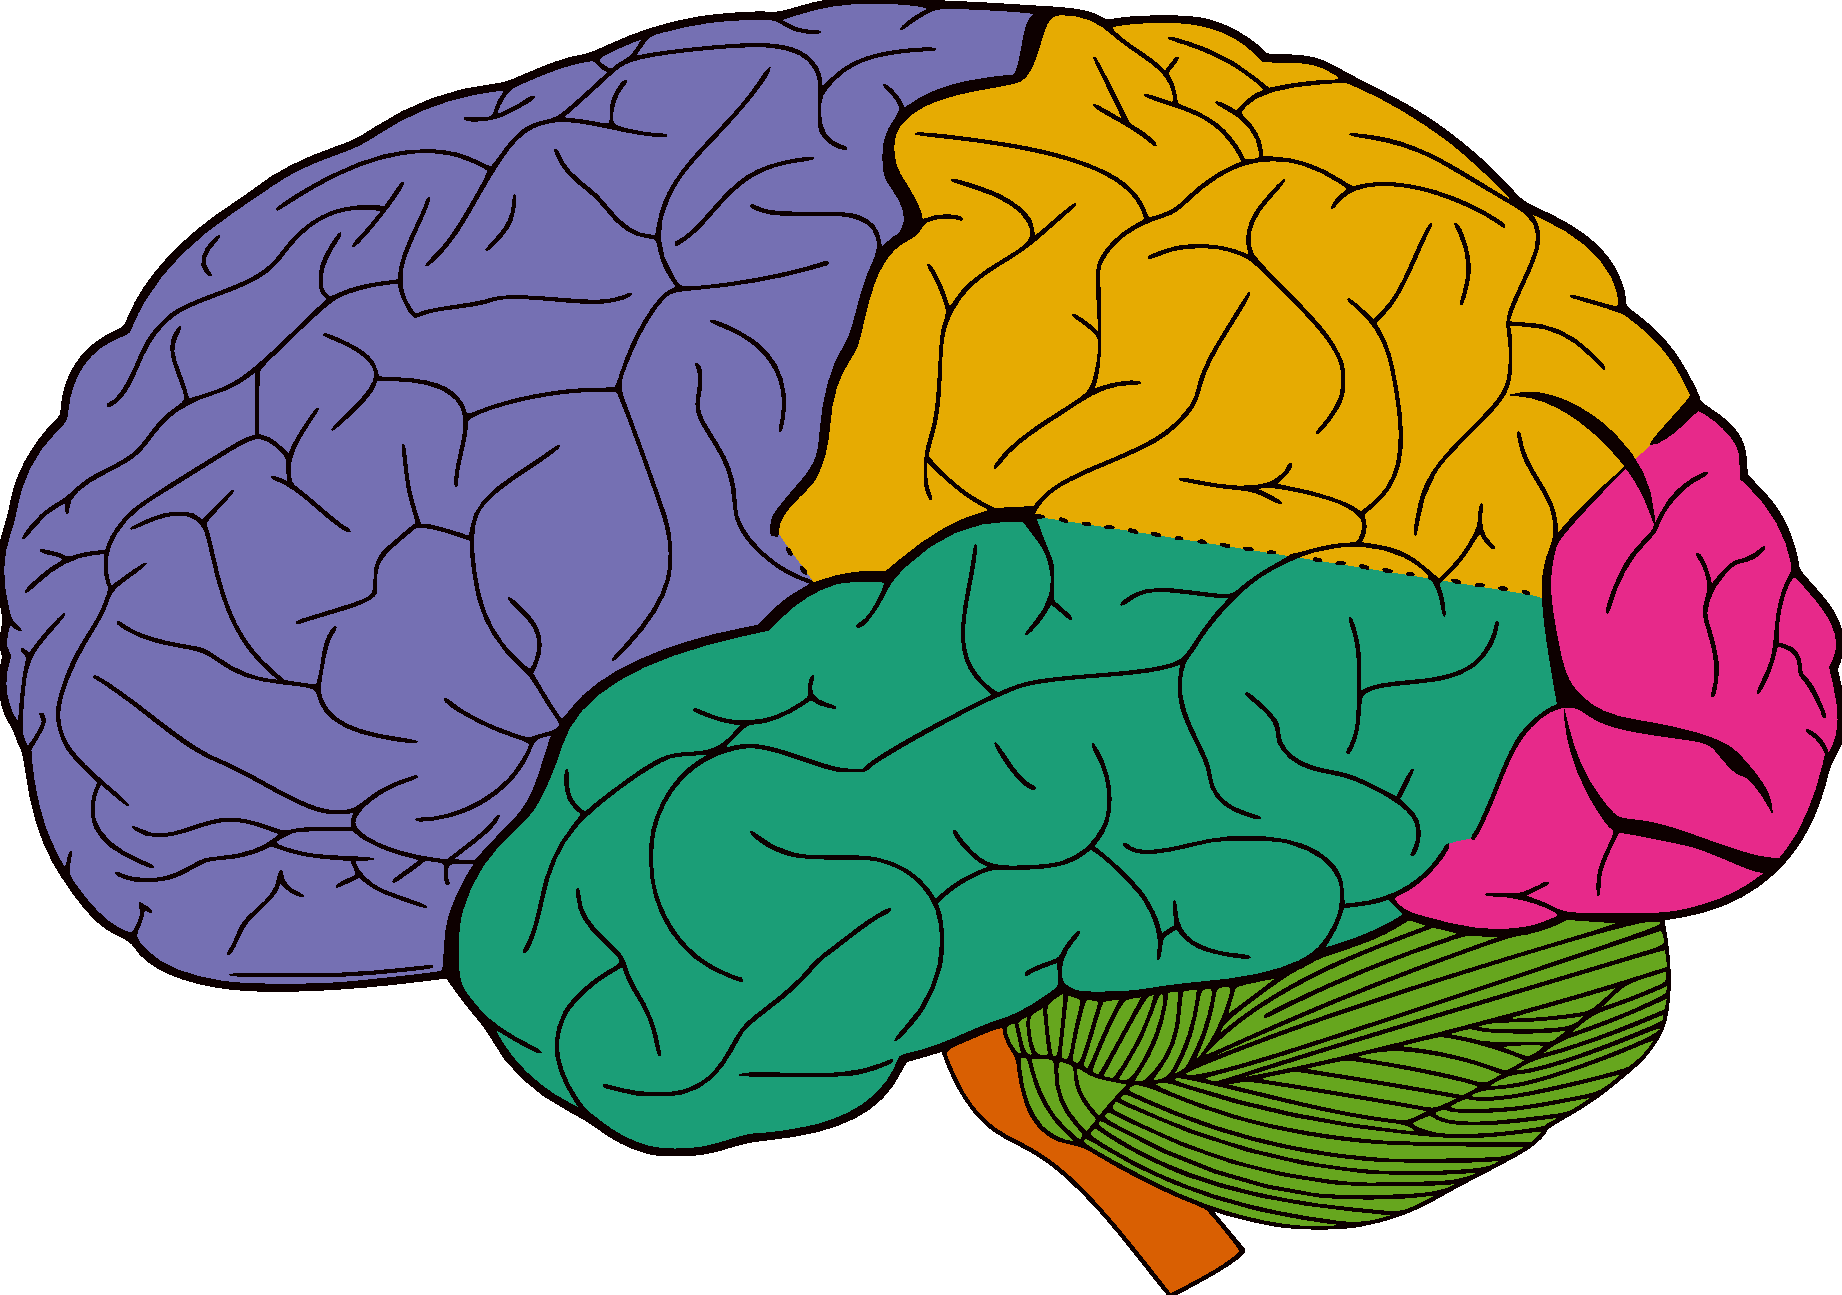
\includegraphics[height=0.3\textwidth]{gfx/neuroanatomy/brain_lobes.pdf}}; %height=4.2cm
        \begin{scope}[overlay]
            \draw[<-] (rel cs:name=fig,x=0.19,y=0.925) -- ++(140:0.66)
                node[anchor=south, pos=1] {\color[RGB]{117,112,179}Lobus frontalis};
            \draw[<-] (rel cs:name=fig,x=0.725,y=0.925) -- ++(42:0.5)
                node[anchor=south, pos=1] {\color[RGB]{230,171,2}Lobus parietalis};
            \draw[<-] (rel cs:name=fig,x=0.95,y=0.75) -- ++(30:0.66)
                node[anchor=south, pos=1] {\color[RGB]{231,41,138}Lobus occipitalis};
            \draw[<-] (rel cs:name=fig,x=0.4,y=0.125) -- ++(210:0.25)
                node[anchor=north, pos=1] {\color[RGB]{27,158,119}Lobus temporalis};
            \draw[<-] (rel cs:name=fig,x=0.95,y=0.2) -- ++(-20:0.66)
                node[anchor=north, pos=1] {\color[RGB]{102,166,30}Cerebellum};
            \draw[<-] (rel cs:name=fig,x=0.281,y=0.315) -- ++(205:1.0)
                node[anchor=north, pos=1] {Sulcus lateralis};
            \draw[<-] (rel cs:name=fig,x=0.4,y=0.87) -- ++(90:1)
                node[anchor=south, pos=1] {Sulcus centralis};
        \end{scope}
        % \path[] ($(fig.south west)-(0,0)$) rectangle ($(fig.north east)+(1,0.75)$);
    \end{tikzpicture}
    }
\hfill
\tikzset{external/export next=false}
\subcaptionbox{%
    \label{fig:coronalStained}%
    Coronal section stained for cell bodies. The \ac{GM} is dark while the \ac{WM} is bright. The left and right hemisphere is connected via the corpus callosum.
    \footnotemark}%
    [\tikzwidth]{
    \tikzset{external/export next=false}
    \begin{tikzpicture}[every node/.style={font=\footnotesize,},]
        \node[inner sep=0pt, anchor = south west] (fig) at (0,0) {\includegraphics[height=0.3\textwidth]{gfx/brain/BB20_4050.png}}; %height=4.2cm
        \begin{scope}[overlay]
            \draw[white, semithick, <-] (rel cs:name=fig,x=0.46,y=0.55) -- ++(-70:0.75);
            \draw[RED, <-] (rel cs:name=fig,x=0.46,y=0.55) -- ++(-70:0.5) node[anchor=north, pos=1] {%
                \shadowoffset{0.25pt}
                \shadowcolor{black!10!white}
                \shadowtext{\color{RED}Corpus callosum}};
            \node at (rel cs:name=fig,x=0.25,y=0.65) {%
                \shadowoffset{0.25pt}
                \shadowcolor{black!10!white}
                \shadowtext{\color{RED}WM}};
            \draw[white, <-] (rel cs:name=fig,x=0.725,y=0.85) -- ++(30:0.5);
            \draw[RED, <-] (rel cs:name=fig,x=0.725,y=0.85) -- ++(30:0.5) node[anchor=west, pos=1] {\color{RED}GM};
        \end{scope}
    \end{tikzpicture}
    }
\caption[]{Illustration of the human brain and a cell body stained coronal section.}
\label{fig:humanBrain}
\end{figure}
\addtocounter{footnote}{-1}\footnotetext{Drawing of the side view showing the B06 brain collection of the \acs{INM-1}.}
\addtocounter{footnote}{+1}\footnotetext{Coronal stained section 4050 from the BigBrain Project \cite{Amunts2013}.}
%
The cerebellum and cerebrum contain a \ac{GM} structure at the brain surface.
This structure is filled with neurons.
These cells have the task of processing the information of all signals coming from inside and outside the brain.
Such cells are arranged in cortical layers that have different thicknesses, cell types, and densities specific to a brain area.
These cells have a relatively high density and are not only locally interconnected with each other, but connect also with different brain areas.
Therefore, the folding of the brain is particularly important to increase the surface and therefore the number of cells.
In the human brain there are several billions of nerve cells.
There are many types of cells, \eg{} granule or pyramidal cells.
The highly interconnected structure and arrangement of the various cells is the source of its high number of different functionalities.
It is important to investigate the human brain to gain a better understanding of the brain's function and an improved understanding of pathophysiological processes that may lead to improved medical treatment of brain diseases.
%
%
%
\section{Nerve Fiber Architecture} \label{sec:fiberArchitecture}
%
A typical nerve cell (see \cref{fig:CortexAndNerveCell}) comprises a cell body, called a soma, that processes incoming information.
The information arrives via dendrites, which are star-shaped branches.
The axon, or nerve fiber, is the cell's information output.
It travels through the brain often associated with nerve fiber bundles to its destination, where it connects with the axon terminal to other neurons.
\par
%
\begin{figure}[!t]
\setlength{\tikzwidth}{0.75\textwidth}
\centering
\tikzset{external/export next=false}
\begin{tikzpicture}[every node/.style={font=\small,},]
    \node[inner sep=0pt, anchor = south west] (fig) at (0,0) {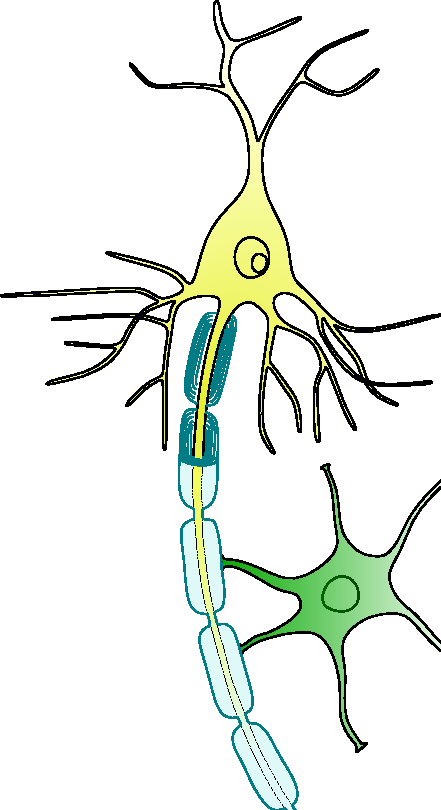
\includegraphics[ angle=90,width=\tikzwidth]{gfx/neuroanatomy/neuron-axon.pdf}}; %height=4.2cm
    \begin{scope}[overlay]
        \node[anchor=south] at (rel cs:name=fig,x=0.72,y=1.025) {Oligodendrocyte};
        \node[anchor=north] at (rel cs:name=fig,x=0.235,y=0.22) {Cell Body};
        \node[anchor=west] at (rel cs:name=fig,x=1,y=0.675) {Axon};
        \node[anchor=north] at (rel cs:name=fig,x=0.7,y=0.4) {Myelin};
        \draw[<-] (rel cs:name=fig,x=0.9,y=0.5) -- ++(-69:0.5) node[pos=1,anchor=north] {Node of Ranvier};
        \draw[<-] (rel cs:name=fig,x=0.295,y=0.53) -- ++(-140:0.75) node[pos=1,anchor=north] {Nucleus};
        \node[anchor=south] at (rel cs:name=fig,x=0.24,y=0.8) (D) {Dendrites};
        \draw[->] (rel cs:name={D},x=0.3,y=0) -- ++(-155:0.6){};
        \draw[->] (rel cs:name={D},x=0.7,y=0) -- ++(-25:0.6){};
    \end{scope}
    \path[] ($(fig.south west)-(0,0)$) rectangle ($(fig.north east)+(1,0.75)$);
\end{tikzpicture}
\caption[]{Illustration of a neuron with axon and oligodendrocytes.
    The oligodendrocyte build up a layered lipid structure, surrounding the axon.
    The myelin layers are separated along the axon by nodes of Ranvier.}
\label{fig:CortexAndNerveCell}
\end{figure}
%
The axon is surrounded by a myelin sheath, a lipid layered structure generated by nearby oligodendrides (see \cref{fig:CortexAndNerveCell}).
The myelin electrically insulates the axon and improves the speed of propagation of the electrical action potential along the axon and also its signal strength.
The diameter of the myelin ranges from about $\SI{0.5}{\micro\meter}$ to several micrometers (see \cref{tab:axonDiameter}).
There are many types of axons.
Some contain a very thick myelin layer, while others have none.
The high density of axons and myelin makes the brain appear white and is therefore called \acreset{WM}\ac{WM}, whereas the outer cell bodies appear darker and is called \acreset{GM}\ac{GM}.
This color difference is clearly visible in a Nissl stained histological sections (see \cref{fig:coronalStained}).
\par
%
To enhance the contrast of the nerve fibers with respect to the background, staining like Nissl is used to darken the myelin (see \cref{fig:brainMyelinStain}).
This allows to follow small nerve fibers down to individual nerves depending on their myelination degree.
Larger nerve fiber bundles are so dark that mostly no orientation can be extracted.
\par
%
\Cref{fig:brainMyelinStain} shows a Nissl stained brain section.
Between neurons, individual nerve fibers form complex reticular structures.
Several nerve fiber bundles traverse the thalamus and can be seen as dark structures.
A closer look with an electron microscope into a nerve fiber bundle of the corpus callosum of a rodent is shown in \cref{fig:elecMic}.
The nerve fibers of the $\SI{100}{\nano\meter}$ thin section are densely packed together.
Axon diameter and myelin thickness vary from nerve fiber to nerve fiber.
%
\begin{figure}[!t]
	\centering
    \tikzset{external/export=false}
    \setlength{\tikzwidth}{0.475\textwidth}
    \subcaptionbox{%
        \label{fig:brainMyelinStain}
        Myelin staining of the human thalamus, sagittal section.
        \textcolor{Orange}{Nerve fiber bundle} structures are visible as elliptical dark shape.
        In between \textcolor{ProcessBlue}{net-like structures} are formed from individual nerve fibers.
        \url{http://brainmaps.org/HBP3/h.sapiens/sag/h5thal-myelin/17a}}
    [\tikzwidth]{
        \begin{tikzpicture}[]
            \node[inner sep=0pt, anchor = south west] (fig) at (0,0)
            {\includegraphics[width=\tikzwidth, trim=281 152 0 0, clip]{gfx/neuroanatomy/NeuralNet-BrainAtlasDotOrg.png}};
            %
            \draw[Orange, ultra thick] (rel cs:name=fig,x=0.42,y=0.49) ellipse (0.75 and 0.375);
            \draw[ProcessBlue, ultra thick] (rel cs:name=fig,x=0.7,y=0.3) ellipse (1.1 and 0.7);
            %
            \draw[white, ultra thick] let
                \p1=(rel cs:name=fig,x=0,y=0),
                \p2=(rel cs:name=fig,x=0.1041,y=0),
                \n1={veclen(\x1-\x2,\y1-\y2)}
            in
                ($(fig.south east)+(-0.2,0.2)$) -- ++ (180:\n1) node[above, midway, anchor=south]{$\SI{50}{\micro\meter}$};
        \end{tikzpicture}   
    }
    \hfill
    \subcaptionbox{%
        \label{fig:elecMic} Electron microscope image of a $\SI{100}{\nano\meter}$ thin section of rodent corpus callosum \cite{WALHOVD20142}.
        The myelin is visible as dark surroundings around the inner axon.}
    [\tikzwidth]{
        \begin{tikzpicture}[]
            \node[inner sep=0pt, anchor = south west] (fig) at (0,0)
            {\includegraphics[width=\tikzwidth]{gfx/brain/elec_micrograph_rodent_cc.jpg}};
            \draw[white, ultra thick] let
                \p1=(rel cs:name=fig,x=0,y=0),
                \p2=(rel cs:name=fig,x=0.1347,y=0),
                \n1={veclen(\x1-\x2,\y1-\y2)}
            in
                ($(fig.south east)+(-0.2,0.2)$) -- ++ (180:\n1) node[above, midway, anchor=south]{$\SI{1}{\micro\meter}$};
        \end{tikzpicture}
    }
\end{figure}
%
%
%
\section{Axon Dimensions}
\label{sec:axonMicroscopy}
%
\Cref{tab:axonDiameter} lists diameters of the nerve fibers in the human brain.
The diameter and their standard deviation are region-specific.
The $g_{\mathit{ratio}}$ describes the fraction of the axon to the entire nerve fiber diameter.
From studies with \ac{dMRI} and electron microscopy the $g_{\mathit{ratio}}$ is in the range of $\SI{0.6}{}$ to $\SI{0.9}{}$, depending on the region (see \cref{tab:gratio}).
%
\begin{table}[!b]
\centering
\pgfplotstabletypeset[
    thesisTableStyle,
    font=\footnotesize,
    columns/area/.style={string type},
    columns/mean/.style={string type},
    columns/std/.style={string type},
]{
    area mean std
    {sup. longitudinal fasc.} $\SI{0.8}{\micro\meter}$ $\SI{0.2}{\micro\meter}$
    {inferior occipital fasc.} $\SI{0.51}{\micro\meter}$ $\SI{0.05}{\micro\meter}$
    {corpus callosum} $\SI{0.69}{\micro\meter}$ $\SI{0.04}{\micro\meter}$
}
\caption[]{Nerve fiber diameter distribution of the human brain.
    Mean values over three human brains \cite{Liewald2014}.}
\label{tab:axonDiameter}
\end{table}
%
\begin{table}[!b]
\centering
\pgfplotstabletypeset[
thesisTableStyle,
font=\footnotesize,
col sep=semicolon,
columns={article,cite,gratio},
columns/article/.style={string type, column name=study, column type = {l}},
columns/cite/.style={string type, column name=reference, column type = {l}},
columns/gratio/.style={string type, column name=$g_{\mathit{ratio}}$},
]{gfx/gratio.csv}
\caption[]{human $g_{\mathit{ratio}}$ from in vivo mri studies.}
\label{tab:gratio}
\end{table}
